\documentclass{beamer}
\usetheme{metropolis}

% specifications for presenter mode
%\beamerdefaultoverlayspecification{<+->}
%\setbeamercovered{transparent}

\usepackage[english]{babel}
\usepackage[utf8x]{inputenc}

%\usepackage{coloremoji}
\usepackage{layout}
\usepackage{multirow}
\usepackage{array}
\usepackage{graphicx}
\graphicspath{ {Figs/} }
\usepackage{animate}

\setbeameroption{show notes}
\setbeamertemplate{note page}[plain]
\usepackage{listings}
\usepackage{datetime}
\usepackage{url}
\usepackage{tcolorbox}
\usepackage{appendixnumberbeamer}

\usepackage{tikz}
\def\checkmark{\tikz\fill[scale=0.4](0,.35) -- (.25,0) -- (1,.7) -- (.25,.15) -- cycle;}

% math shorthand
\usepackage{bm}
\usepackage{amstext}
\usepackage{amsthm}
\usepackage{amsmath}
\usepackage{mathtools}
\newcommand{\R}{\mathbb{R}}
\newcommand{\D}{\mathcal{D}}
\newcommand{\E}{\mathbb{E}}
\newcommand{\I}{\mathbb{I}}
\newcommand{\pr}{\mathbb{P}}
\newcommand{\F}{\mathcal{F}}
\newcommand{\X}{\mathcal{X}}
\newcommand{\M}{\mathcal{M}}
\newcommand{\lik}{\mathcal{L}}

\newtheorem*{assumption*}{\assumptionnumber}
\providecommand{\assumptionnumber}{}
\makeatletter
\newenvironment{assumption}[2]
 {%
  \renewcommand{\assumptionnumber}{Assumption #1: $\mathcal{#2}$}%
  \begin{assumption*}%
  \protected@edef\@currentlabel{#1: $\mathcal{#2}$}%
 }
 {%
  \end{assumption*}
 }
\makeatother

\DeclarePairedDelimiterX{\infdivx}[2]{(}{)}{%
  #1\;\delimsize\|\;#2%
}
\newcommand{\infdiv}{D\infdivx}
\DeclarePairedDelimiter{\norm}{\lVert}{\rVert}
\DeclareMathOperator*{\argmin}{arg\,min}
\DeclareMathOperator*{\argmax}{arg\,max}

% indepndence notation macro
\newcommand\indep{\protect\mathpalette{\protect\independenT}{\perp}}
\def\independenT#1#2{\mathrel{\rlap{$#1#2$}\mkern2mu{#1#2}}}

% Bibliography
\usepackage{natbib}
\bibpunct{(}{)}{,}{a}{}{;}
\usepackage{bibentry}

\title{\normalsize Mediation analysis with stochastic interventions}

\author{\href{https://nimahejazi.org}{Nima Hejazi}\\[-10pt]}

\institute{
  \begin{figure}[!htb]
    \centering
    \begin{minipage}{.65\textwidth}
        Graduate Group in Biostatistics, and \\
        Center for Computational Biology, \\
        University of California, Berkeley \\[6pt]
        
\includegraphics[scale=0.12]{twitter-icon.png}
          \href{https://twitter.com/nshejazi}{nshejazi} \\
        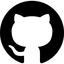
\includegraphics[scale=0.09]{github-icon.png}
          \href{https://github.com/nhejazi}{nhejazi} \\
        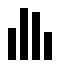
\includegraphics[scale=0.12]{homepage.png}
          \href{https://nimahejazi.org}{nimahejazi.org} \\
        
\includegraphics[scale=0.12]{pdf-icon.png}
        \href{https://bit.ly/2020\_acic\_mediate}{bit.ly/2020\_acic\_mediate} \\
        {\scriptsize joint work with Iv\'an D\'iaz and Mark van der Laan}
    \end{minipage}%
    \begin{minipage}{0.35\textwidth}
      \centering
      
\includegraphics[height=0.80in,width=0.80in]{ucberkeleyseal_874_540.eps}
    \end{minipage}
  \end{figure}
}

\date{\today}

%%%%%%%%%%%%%%%%%%%%%%%%%%%%%%%%%%%%%%%%%%%%%%%%%%%%%%%%%%%%%%%%%%%%%%%%%%%%%%%%

\begin{document}

\begin{frame}[noframenumbering]
  \thispagestyle{empty}
  \titlepage
\end{frame}

%%%%%%%%%%%%%%%%%%%%%%%%%%%%%%%%%%%%%%%%%%%%%%%%%%%%%%%%%%%%%%%%%%%%%%%%%%%%%%%%

\begin{frame}[c]{Stochastic Population Intervention (In)Direct Effects}

\begin{center}
\begin{itemize}
\itemsep0.25pt
\item Consider $O = (W, A, Z, Y) \sim P_0 \in \mathcal{M}$, for $W$ a set of
  baseline covariates, $A$ an intervention, $Y$ the outcome, and $Z$ a mediator
  between $A$ and $Y$, with no assumptions on nonparametric model $\mathcal{M}$.
\item We decompose the total population intervention effect (PIE) in terms of a
  \textit{population intervention direct effect (PIDE)} and a \textit{population
  intervention indirect effect (PIIE)}:
  \begin{equation*}
    \psi(\delta) = \overbrace{\mathbb{E}\{Y(A_\delta, Z(A_\delta)) -
       Y(A_\delta, Z)\}}^{\text{PIIE}} + \overbrace{\mathbb{E}\{Y(A_\delta, Z)
       - Y(A, Z)\}}^{\text{PIDE}}.
  \end{equation*}
\item We show causal parameter $\mathbb{E}\{Y(A_\delta, Z)\}$ is identified by a
  functional of the distribution of $O$ \cite{diaz2019causal}:
  \begin{equation*}
    \theta(\delta) = \int m(z, a, w)g_{\delta}(a\mid w)p(z,w) d\nu(a,z,w),
  \end{equation*}
  for outcome mechanism $m(z,a,w)$ and post-intervention treatment mechanism
  $g_{\delta}(a\mid w)$ --- a stochastic intervention drawing
  $A_{\delta} \sim g_{\delta}(a \mid w)$ while letting mediator $Z$ take on its
  natural value.
\end{itemize}
\end{center}

\note{
}

\end{frame}

%%%%%%%%%%%%%%%%%%%%%%%%%%%%%%%%%%%%%%%%%%%%%%%%%%%%%%%%%%%%%%%%%%%%%%%%%%%%%%%%

\begin{frame}[c]{Stochastic Population Intervention (In)Direct Effects}

\begin{center}
\begin{itemize}
\itemsep0.25pt
\item Letting $\eta = (g, e, m, \phi)$, the efficient influence function for
  $\theta(\delta)$ in the nonparametric model $\mathcal{M}$ is
  $D^Y_{\eta, \delta}(o) + D^A_{\eta, \delta}(o) + D^{Z, W}_{\eta, \delta}(o) -
  \theta(\delta)$ for
  \vspace{-0.5em}
  \begin{align*}
    D^{Z, W}_{\eta, \delta}(o) &= \int m(z, a, w) g_{\delta}(a \mid w)
      d\kappa(a),
    \quad
    D^Y_{\eta, \delta}(o) = \mathbf{\textcolor{blue}{\frac{g_{\delta}(a \mid w)}
      {e(a \mid z, w)}}} \{y - m(z,a,w) \},\\
    D^A_{\eta,\delta}(o) &= \frac{\mathbf{\textcolor{red}{\delta\phi(w)}}\{a -
      g(1 \mid w)\}}{\mathbf{\textcolor{red}{\{\delta g(1 \mid w) +
      g(0 \mid w)\}^2}}},
    \quad
    \phi(w) = \mathbb{E}\left\{m(1, Z, W) - m(0, Z, W) \mid W = w \right\},
  \end{align*}
  where, for simplicity, we present the case $A \in \{0, 1\}$. For an unabridged
  treatment, see \cite{diaz2019causal}.
\end{itemize}
\end{center}

\note{
}

\end{frame}

%%%%%%%%%%%%%%%%%%%%%%%%%%%%%%%%%%%%%%%%%%%%%%%%%%%%%%%%%%%%%%%%%%%%%%%%%%%%%%%%

\begin{frame}[c]{Mediation analysis with stochastic interventions}

\begin{center}
\begin{itemize}
  \item To avoid entropy conditions on initial estimators, we rely on
    cross-validation \citep{zheng2011cross, chernozhukov2016double}, letting
    $\hat{\eta}_{j}$ be the estimator of $\eta = (g, e, m, \phi)$ and $j(i)$ the
    index of the validation set containing observation $i$.
  \item A targeted minimum loss estimator (TMLE) may be constructed by using the
    efficient influence function to update components of the substitution
    estimator via a targeting procedure:
    \begin{equation*}
      \hat{\theta}_{\text{TMLE}}(\delta) = \int \frac{1}{n} \sum_{i=1}^n
      \hat{m}^{\star}_{j(i)}(Z, a, W)
      \hat{g}_{\delta, j(i)}^{\star}(a \mid W) d\kappa(a).
    \end{equation*}
\end{itemize}
\end{center}

\note{
}

\end{frame}


%%%%%%%%%%%%%%%%%%%%%%%%%%%%%%%%%%%%%%%%%%%%%%%%%%%%%%%%%%%%%%%%%%%%%%%%%%%%%%%%

\begin{frame}[c]{Mediation analysis with stochastic interventions}

\begin{center}
\begin{itemize}
  \itemsep10pt
  \item $\hat{g}_{\delta}^{\star}(a \mid w)$ and $\hat{m}^{\star}(z,a,w)$ are
    generated via \textit{targeting} fluctuation regressions that tilt initial
    estimates towards solutions of scores
    $\frac{1}{n}\sum_{i=1}^n D^A(O_i) = 0$ and
    $\frac{1}{n}\sum_{i=1}^n D^Y(O_i) = 0$, respectively.
    %$\text{logit}(\hat{g}_{\delta,k\xi}) =
    %\text{logit}(\hat{g}_{\delta,(k-1)\xi}) + \xi_{\Delta g}^{\text{lfm}}
    %\mathbf{\textcolor{red}{H^A_{(k-1)\xi}}}$ and
    %$\text{logit}(\hat{m}_{k\xi}) = \text{logit}(\hat{m}_{(k-1)\xi}) +
    %\xi_{\Delta m}^{\text{lfm}}
    %\mathbf{\textcolor{blue}{H^Y_{(k-1)\xi}}}$.
    \begin{itemize}
      \item Unlike the one-step estimator, TMLE constructs a substitution
        estimator, respecting bounds.
      \item Targeting step uses the method of universal least favorable
        one-dimensional submodels \citep{vdl2016one}.
    \end{itemize}
\end{itemize}
\end{center}

\note{
}

\end{frame}

%%%%%%%%%%%%%%%%%%%%%%%%%%%%%%%%%%%%%%%%%%%%%%%%%%%%%%%%%%%%%%%%%%%%%%%%%%%%%%%%

\begin{frame}[c]{Software implementation}

\begin{center}
\begin{itemize}
  \setlength\itemsep{0.5em}
  \item The \underline{\texttt{medshift} \texttt{R} package}
    \cite{hejazi2019medshift} implements these estimators and leverages
    state-of-the-art machine learning in the procedure.
    \begin{itemize}
      \item Construction of all estimators via the eponymous \texttt{medshift()}
        function.
      \item Uses the \texttt{sl3} \texttt{R} package to incorporate machine
        learning facilities.
      \item Relies on the framework of the \texttt{tmle3} \texttt{R} package for
        TMLE implementation.
      \item Flexible cross-fitting implementation via the \texttt{origami}
        \texttt{R} package.
    \end{itemize}
  \item \texttt{sl3}, \texttt{tmle3}, and \texttt{origami} are core engines of
    the new \textbf{\texttt{tlverse}} software ecosystem.
    \begin{itemize}
      \item Check out \url{https://tlverse.org}
      \item Our handbook: \url{https://tlverse.org/tlverse-handbook}
    \end{itemize}
\end{itemize}
\end{center}

\note{
}

\end{frame}

%%%%%%%%%%%%%%%%%%%%%%%%%%%%%%%%%%%%%%%%%%%%%%%%%%%%%%%%%%%%%%%%%%%%%%%%%%%%%%%%

% don't want dimming with references
\setbeamercovered{}
\beamerdefaultoverlayspecification{}

\begin{frame}[c,allowframebreaks]{}

\scriptsize
\bibliographystyle{apalike}
\bibliography{references}

\end{frame}

%%%%%%%%%%%%%%%%%%%%%%%%%%%%%%%%%%%%%%%%%%%%%%%%%%%%%%%%%%%%%%%%%%%%%%%%%%%%%%%%

\begin{frame}[c]{Thank you.}

\large
Slides: \href{http://bit.ly/2020\_acic\_mediate}{bit.ly/2020\_acic\_mediate}
  \quad

\includegraphics[height=4mm]{Figs/cc-zero.png}

\vspace{2mm}
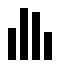
\includegraphics[scale=0.14]{homepage.png} \url{https://nimahejazi.org}

\vspace{2mm}
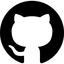
\includegraphics[scale=0.11]{github-icon.png}
  \url{https://github.com/nhejazi}

\vspace{2mm}

\includegraphics[scale=0.14]{twitter-icon.png}
  \url{https://twitter.com/nshejazi}

\end{frame}

%%%%%%%%%%%%%%%%%%%%%%%%%%%%%%%%%%%%%%%%%%%%%%%%%%%%%%%%%%%%%%%%%%%%%%%%%%%%%%%%

%\appendix
%\begin{frame}[standout]
  %Appendix
%\end{frame}

%%%%%%%%%%%%%%%%%%%%%%%%%%%%%%%%%%%%%%%%%%%%%%%%%%%%%%%%%%%%%%%%%%%%%%%%%%%%%%%%

%\begin{frame}[c]{Nonparametric Conditional Density Estimation}

%\begin{center}
%\begin{itemize}
  %\itemsep8pt
  %\item To compute the auxiliary covariate $H(a,w)$, we need to estimate
    %conditional densities $g(A \mid W)$ and $g(A - \delta \mid W)$.
  %\item There is a rich literature on density estimation, we follow the approach
    %proposed in \cite{diaz2011super}.
  %\item To build a conditional density estimator, consider
    %\begin{equation*}
      %g_{n, \alpha}(a \mid W) = \frac{\pr (A \in [\alpha_{t-1}, \alpha_t)
        %\mid W)}{\alpha_t - \alpha_{t-1}},
    %\end{equation*}
    %for $\alpha_{t-1} \leq a < \alpha_t$.
    %\vspace{0.5em}
    %\begin{itemize}
      %\itemsep4pt
      %\item This is a classification problem, where we estimate the probability
        %that a value of $A$ falls in a bin $[\alpha_{t-1}, \alpha_t)$.
      %\item The choice of the tuning parameter $t$ corresponds roughly to the
        %choice of bandwidth in classical kernel density estimation.
    %\end{itemize}
%\end{itemize}
%\end{center}

%\note{
%}

%\end{frame}

%%%%%%%%%%%%%%%%%%%%%%%%%%%%%%%%%%%%%%%%%%%%%%%%%%%%%%%%%%%%%%%%%%%%%%%%%%%%%%%%

\end{document}
